% Compile on "nestor" which has the latest LaTeX distribution.
%    pdflatex brainbrowser-hbm2011poster.tex
%
\documentclass[a4shrink]{baposter}
%\documentclass[showframe]{baposter}
%\documentclass{baposter}

% \usepackage[vlined]{algorithm2e}
\usepackage{times}
\usepackage{calc}
\usepackage{url}
\usepackage{graphicx}
\usepackage{relsize}
\usepackage{multirow}
\usepackage{booktabs}
\usepackage{wrapfig}
\usepackage{floatflt}

\usepackage{graphicx}
\usepackage{multicol}
\usepackage[T1]{fontenc}
\usepackage{ae}

%\usepackage{helvet}
%\usepackage{bookman}
%\usepackage{palatino}

\graphicspath{{images/}}

%%%%%%%%%%%%%%%%%%%%%%%%%%%%%%%%%%%%%%%%%%%%%%%%%%%%%%%%%%%%%%%%%%%%%%%%%%%%%%%%
% Multicol Settings
%%%%%%%%%%%%%%%%%%%%%%%%%%%%%%%%%%%%%%%%%%%%%%%%%%%%%%%%%%%%%%%%%%%%%%%%%%%%%%%%
\setlength{\columnsep}{0.7em}
\setlength{\columnseprule}{0mm}

%%%%%%%%%%%%%%%%%%%%%%%%%%%%%%%%%%%%%%%%%%%%%%%%%%%%%%%%%%%%%%%%%%%%%%%%%%%%%%%%
% Save space in lists. Use this after the opening of the list
%%%%%%%%%%%%%%%%%%%%%%%%%%%%%%%%%%%%%%%%%%%%%%%%%%%%%%%%%%%%%%%%%%%%%%%%%%%%%%%%
\newcommand{\compresslist}{%
\setlength{\itemsep}{1pt}%
\setlength{\parskip}{0pt}%
\setlength{\parsep}{0pt}%
}

\newcommand{\Frac}[2]{\displaystyle{\frac{\displaystyle{#1}}
                                         {\displaystyle{#2}}}}
\newcommand{\Sum}[2]{\displaystyle{\sum_{#1}^{#2}}}

%%%%%%%%%%%%%%%%%%%%%%%%%%%%%%%%%%%%%%%%%%%%%%%%%%%%%%%%%%%%%%%%%%%%%%%%%%%%%%
%%% Begin of Document
%%%%%%%%%%%%%%%%%%%%%%%%%%%%%%%%%%%%%%%%%%%%%%%%%%%%%%%%%%%%%%%%%%%%%%%%%%%%%%

\begin{document}

\begin{poster}{
  grid=no,            % Show grid to help with alignment
  colspacing=1em,     % Column spacing
  headerColorOne=cyan!20!white!90!black,    % Color style
  borderColor=cyan!30!white!90!black,
  textborder=faded,                         % Format of textbox
  headerborder=open,                        % Format of text header
  headershape=roundedright,
  background=none,
  bgColorOne=cyan!10!white,
  headerheight=0.20\textheight,
  background=none,
  headershade=plain}%
%
% Eye Catcher
{}
%
% Title
{\sf\Huge BrainBrowser\\
    \huge Web-Based 3D Visualization for the MACACC Dataset and Other Surface Data \\
    \vspace{0.25em}
    \large {\tt{http://brainbrowser.cbrain.mcgill.ca/}}
    \vspace{0.25em}}
%
%
%
% Authors
{\sf\normalsize Nicolas Kassis, Gaolang Gong, Marc-Etienne Rousseau, Reza~Adalat and Alan~Evans\\
\small Montreal Neurological Institute, McGill University, Montr\'{e}al, 
       Qu\'{e}bec, Canada \\
    \vspace{0.25em}
  %%{\includegraphics[width=0.32\linewidth]{cbrain_logos.png}}
    \vspace{-3em}
}
%
% logos empty on right margin
{}

% Width of left inset image
% \setlength{\leftimgwidth}{0.78em+8.0em}

%%%%%%%%%%%%%%%%%%%%%%%%%%%%%%%%%%%%%%%%%%%%%%%%%%%%%%%%%%%%%%%%%%%%%%%%%%%%%%
%%% Now define the boxes that make up the poster
%%%---------------------------------------------------------------------------
%%% Each box has a name and can be placed absolutely or relatively.
%%% The only inconvenience is that you can only specify a relative position 
%%% towards an already declared box. So if you have a box attached to the 
%%% bottom, one to the top and a third one which should be in between, you 
%%% have to specify the top and bottom boxes before you specify the middle 
%%% box.
%%%%%%%%%%%%%%%%%%%%%%%%%%%%%%%%%%%%%%%%%%%%%%%%%%%%%%%%%%%%%%%%%%%%%%%%%%%%%%

%%%%%%%%%%%%%%%%%%%%%%%%%%%%%%%%%%%%%%%%%%%%%%%%%%%%%%%%%%%%%%%%%%%%%%%%%%%%%%
\headerbox{Introduction}{name=introduction,column=0,span=1.5,row=0}{
BrainBrowser is web-based, 3D visualization tool for neuroimaging. Using web-standard technologies, such as WebGL and HTML5, it allows for real time manipulation and analysis of 3D neuroimaging data whether it be models provided by the user, or precalculated maps, such as the MACACC data set (Mapping Anatomical Correlations Across Cerebral Cortex). MACACC was previously proposed to characterize vertex-wise correlations of any cortical morphological descriptor (cortical thickness, area and volume) across subjects. The correlations represent structural associations between a seed vertex and all other vertices.  We have now created a database of correlation maps for all surface vertices.\vspace{0.3em}

\begin{center}
  \begin{tabular}{cc}
    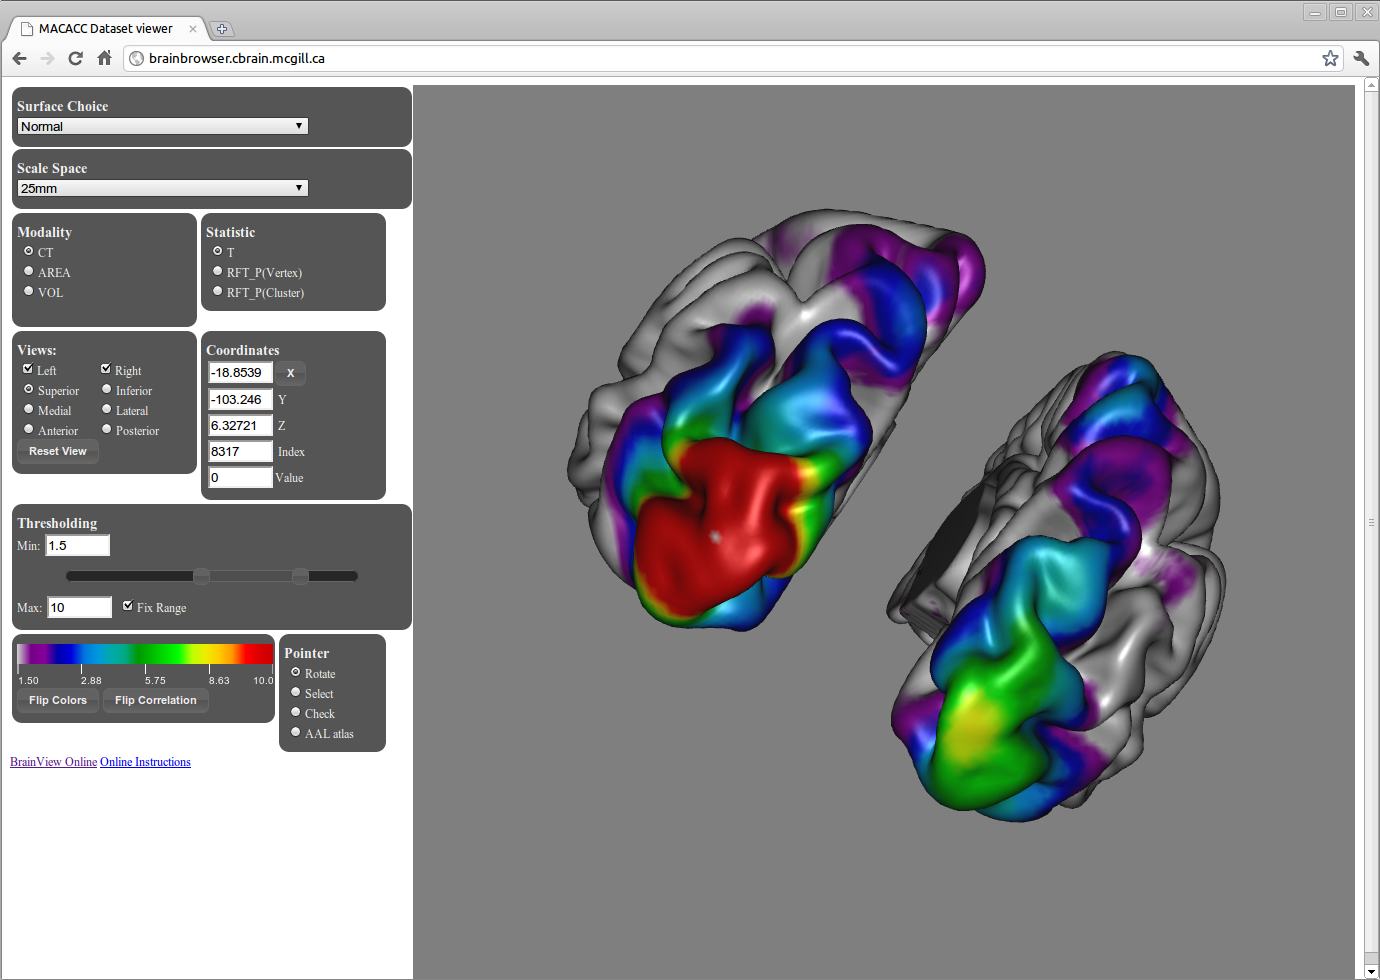
\includegraphics[width=0.95\linewidth]{macacc.png}
  \end{tabular}
\end{center}
\begin{center}
  \begin{tabular}{cc}
    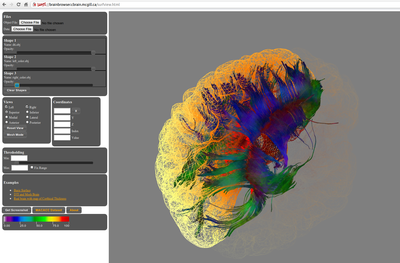
\includegraphics[width=0.95\linewidth]{brainbrowser.png}
  \end{tabular}
\end{center}

}

%%%%%%%%%%%%%%%%%%%%%%%%%%%%%%%%%%%%%%%%%%%%%%%%%%%%%%%%%%%%%%%%%%%%%%%%%%%%%%

\headerbox{BrainBrowser}{name=brainbrowser,column=1.5,span=1.5, row=0}{
BrainBrowser uses cutting-edge technologies such as WebGL and HTML5, which allow for the rendering and manipulation of 3D models within a web browser. These technologies are built into the latest versions of several popular browsers such as Chrome  and Firefox. Any user with access to the Internet is now able to visualize their data without any requirements for complex software installation or local configuration.
\linebreak
BrainBrowser can be used to visualize all kinds of 3D objects. Currently, BrainBrowser is currently targeted at visualizing brain surfaces extracted from MRI data and 3D fibre pathways derived from DTI. The 3D models can be rotated, translated and zooming is also possible. BrainBrowser reads the geometry of these objects from MNI Object files (.obj) and can be adapted to understand data in other formats as well. 
\linebreak 
 For brain surfaces, data associated with each vertex is mapped to a color space and displayed on the 3D model. These datasets can be either provided as text files with one value per vertex or directly as MINC or NIFTI volumes. If a dataset is supplied in MINC or NIFTI format, BrainBrowser will project the data onto the surface using the volume\_object\_evaluate program of the MINC toolkit. This is useful for datasets such as cortical thickness, FMRI activation maps, etc. The thresholds can be adjusted to make values of interest more visible.  
\linebreak
BrainBrowser is built on top of WebGL. WebGL was created to provide an interface between JavaScript, used for web-programming, and the OpenGL API, commonly used for 3D modelling. WebGL has recently been ratified by the W3C, meaning that it is now a web standard. This allows BrainBrowser to work seamlessly across platforms (Windows, Mac OSX, Linux) and across various popular browsers. Currently, Chrome and Firefox support WebGL, while support is planned for upcoming versions Safari and Opera. Internet Explorer can support WebGL using the Chrome Frames extension provided by Google.

}

\headerbox{MACACC}{name=macacc,column=1.5,span=1.5,below=brainbrowser}{
BrainBrowser includes access to the MACACC dataset which is used to explore structural correlations across the cortex, derived in database of 152 young normal subjects from the International Consortium for Brain Mapping (ICBM, Mazziotta J et al., 2001). Cortical thickness at each of 80K 3D locations were calculated using the CLASP algorithm (MacDonald D et al., 2000; Kim JS et al., 2005). This subject population is the same as used for the MNI152 stereotaxic voxelwise templates used, for instance, in SPM. Structural correlation maps are calculated according to the procedures in Lerch et al., (2005), wherein the correlation across subjects, between the cortical thickness at a seed vertex and at any other vertex, is measured. This yields a cortical thickness correlation map for that seed vertex. The BrainBrowser database contains maps for all cortical vertices for each of three vertexwise morphological variables (thickness, area, volume). Furthermore, since the blurring kernel used will profoundly alter the derived statistical map, the results are generated for 9 different surface-blurring kernels and for three different statistics. In total, the BrainBrowser database comprises ~6.3 million maps for the following permutations: 80K vertices x 9 blurring kernels x 3 morphological indices x 3 statistical.

}





%%%%%%%%%%%%%%%%%%%%%%%%%%%%%%%%%%%%%%%%%%%%%%%%%%%%%%%%%%%%%%%%%%%%%%%%%%%%%%
\headerbox{References}{name=references,column=0,span=3.0,below=macacc}{
  
  \begin{itemize} \tiny
    \item \tiny Kim JS. et al., 2005, Automated 3-D extraction and evaluation of the inner and outer cortical surfaces using a Laplacian map and partial volume effect classification, NeuroImage Volume 27, Issue 1, 1 August 2005, Pages 210-221
    \item \tiny Lerch J. et al.,  2006,  Mapping anatomical correlations across cerebral cortex (MACACC) using cortical thickness from MRI, NeuroImage, Volume 31, Issue 3, 1 July 2006, Pages 993-1003
    \item \tiny Lyttelton O. et al, 2007, An unbiased iterative group registration template for cortical surface analysis, NeuroImage Volume 34, Issue 4, 15 February 2007, Pages 1535-1544
    \item \tiny MacDonald D. et al., 2000,  Automated 3-D Extraction of Inner and Outer Surfaces of Cerebral Cortex from MRI, NeuroImage Volume 12, 2000,Pages 340–356, 
    \item \tiny Mazziotta J et al., 2001, A probabilistic atlas and reference system for the human brain: International Consortium for Brain Mapping (ICBM), Philosophical Transactions of the Royal Socity, Bological Sciences, August 2001 vol. 356 no. 1412 1293-1322
    \item \tiny MNI Object File format https://brainbrowser.cbrain.mcgill.ca/documentation/mni\_obj\_format.pdf
    \item \tiny WebGL http://khronos.org/webgl/wiki/Main\_Page
  \end{itemize}
}

\end{poster}
\end{document}
